\chapter{Intermoleculaire krachten en oplosmiddelen}\label{ch:b1:intermolecular-forces-solvents}

Een gekko rent tegen een ruit op en hangt eraan aan één teen; geen lijm,
geen zuignap, alleen de aantrekking tussen de moleculen van zijn
teenkussentjes en die van het glas. Water, een molecuul dat lichter is
dan koolstofdioxide, kookt bij \qty{100}{\celsius}, terwijl
koolstofdioxide bij kamertemperatuur een gas is. Olie drijft op azijn en
mengt er nooit mee; keukenzout lost op in water en niet in benzine. Al die
feiten worden niet bepaald door de bindingen binnen de moleculen, maar
door de veel zwakkere krachten ertussen. Dit hoofdstuk deelt die krachten
in, meet hun invloed op kookpunten, en gebruikt ze om een oplosmiddel te
kiezen.

% ledger: bp:H2O (the hook's 100 degC)


\begin{recall}
Boek 1 (jaar 11) introduceerde vanderwaalskrachten en \omterm{def:b1:intermolecular-forces-solvents:hbond}{waterstofbruggen},
en legde uit dat ionaire vaste stoffen oplossen door dissociatie en
\omterm{def:b1:intermolecular-forces-solvents:dissolution}{solvatatie}. \omterm{def:b1:lewis-resonance-vsepr:dipole}{Dipoolmomenten} werden gedefinieerd in
\cref{def:b1:lewis-resonance-vsepr:dipole} en de \omterm{def:b1:periodicity:polarisability}{polariseerbaarheid} in
\cref{def:b1:periodicity:polarisability}. Uit de natuurkunde gebruiken we
de wet van Coulomb: twee ladingen $q_1$ en $q_2$ op een afstand $r$ in
vacuüm trekken elkaar aan of stoten elkaar af met een kracht met norm
$|q_1q_2|/(4\pi
\varepsilon_0 r^2)$.
\end{recall}

\begin{omfigure}
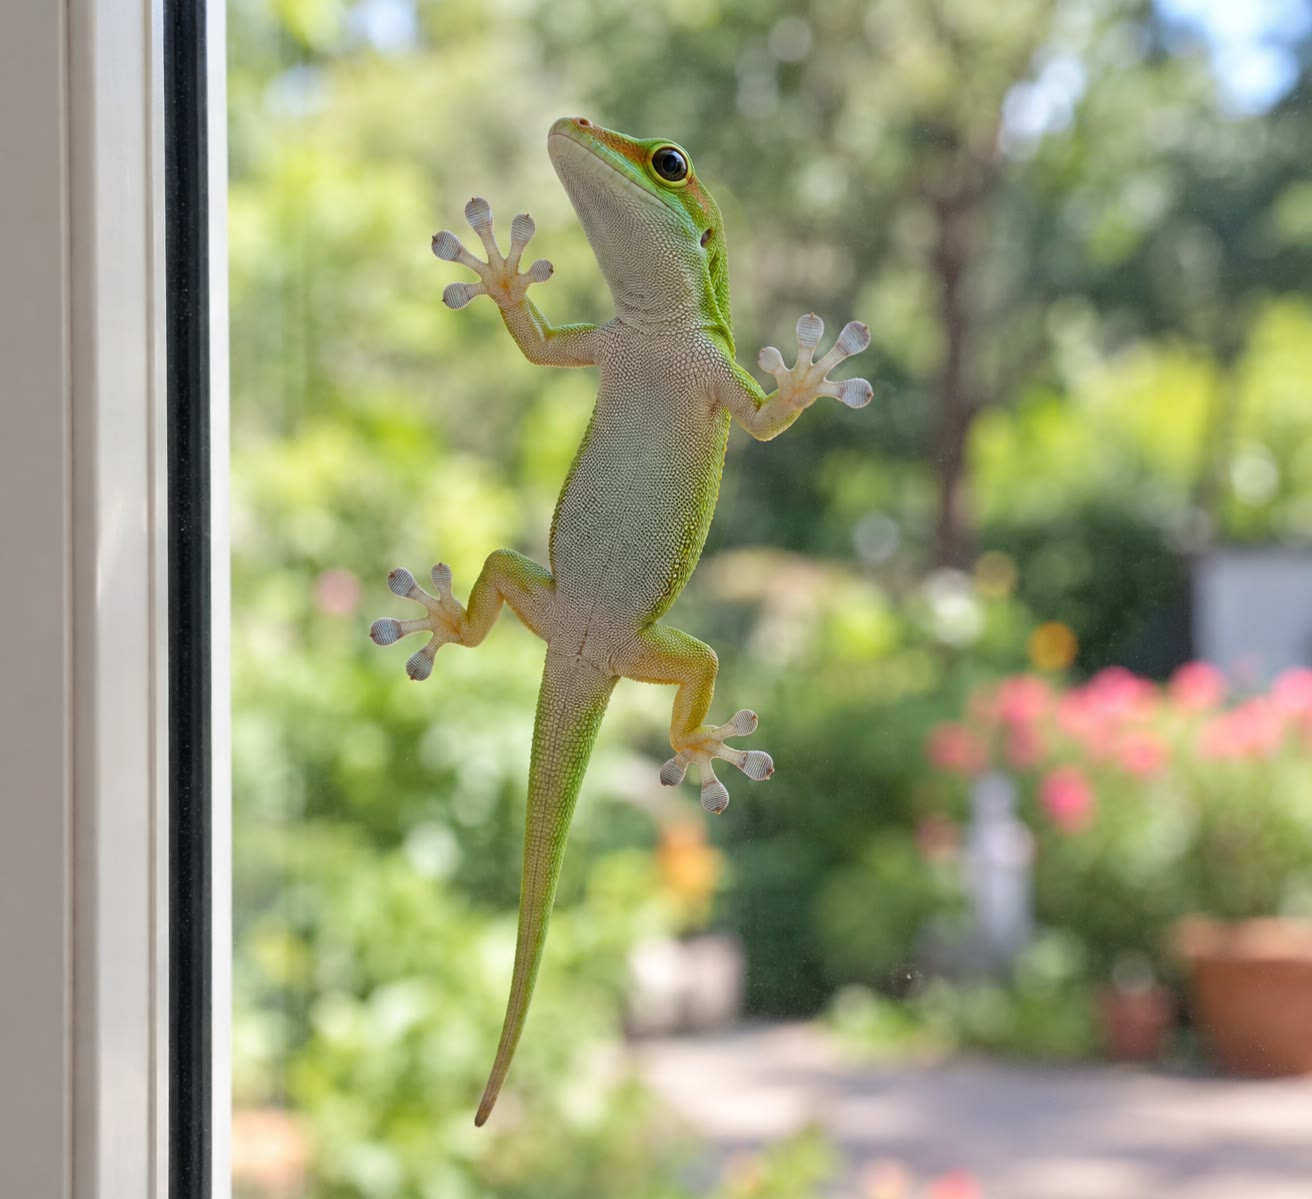
\includegraphics[width=0.52\linewidth]{images/book2/ai/b1-04-gecko.jpg}

{\small Een gekko op een ruit. De miljoenen fijne haartjes van zijn
teenkussentjes komen zo dicht bij het glas dat de zwakke aantrekking
tussen hun moleculen en die van het glas samen groter wordt dan zijn
gewicht.}
\end{omfigure}

\section{Vanderwaalsinteracties}

\begin{definition}[Vanderwaalsinteracties]\label{def:b1:intermolecular-forces-solvents:vdw}
De \emph{vanderwaalsinteracties}\index{vanderwaalsinteractie} zijn de
aantrekkingen tussen neutrale moleculen die voortkomen uit de
wisselwerking van hun dipolen. Er worden drie soorten onderscheiden:
\begin{itemize}
  \item de \emph{keesominteractie}\index{keesominteractie} (of
        oriëntatie-interactie) tussen twee permanente dipolen, die de
        neiging hebben zich kop aan staart te richten;
  \item de \emph{debye-interactie}\index{debye-interactie} (of
        inductie-interactie) tussen een permanente dipool en de dipool
        die hij induceert in een polariseerbare buur;
  \item de \emph{londoninteractie}\index{londoninteractie} (of
        dispersie-interactie) tussen de momentane dipolen die de
        fluctuaties van de elektronenwolken in elk tweetal atomen of
        moleculen veroorzaken, polair of niet, en die elkaar induceren.
\end{itemize}
\end{definition}

\begin{omfigure}
\begin{tikzpicture}[font=\small, >={Stealth},
    mol/.style={draw=black!60, fill=#1, ellipse, minimum width=1.5cm, minimum height=0.8cm}]
  % Keesom
  \node[mol=omDef!20] (a) at (0,0) {}; \node[mol=omDef!20] (b) at (1.7,0) {};
  \node at (-0.45,0) {$\delta^-$}; \node at (0.45,0) {$\delta^+$};
  \node at (1.25,0) {$\delta^-$}; \node at (2.15,0) {$\delta^+$};
  \node[below, align=center] at (0.85,-0.65) {Keesom:\\twee permanente dipolen};
  % Debye
  \begin{scope}[xshift=4.6cm]
    \node[mol=omDef!20] at (0,0) {}; \node[mol=black!5, dashed] at (1.7,0) {};
    \node at (-0.45,0) {$\delta^-$}; \node at (0.45,0) {$\delta^+$};
    \node[omProp] at (1.25,0) {$\delta^-$}; \node[omProp] at (2.15,0) {$\delta^+$};
    \node[below, align=center] at (0.85,-0.65) {Debye:\\permanent en geïnduceerd};
  \end{scope}
  % London
  \begin{scope}[xshift=9.2cm]
    \node[mol=black!5, dashed] at (0,0) {}; \node[mol=black!5, dashed] at (1.7,0) {};
    \node[omProp] at (-0.45,0) {$\delta^-$}; \node[omProp] at (0.45,0) {$\delta^+$};
    \node[omProp] at (1.25,0) {$\delta^-$}; \node[omProp] at (2.15,0) {$\delta^+$};
    \node[below, align=center] at (0.85,-0.65) {London:\\twee momentane dipolen};
  \end{scope}
\end{tikzpicture}

{\small De drie \omterm{def:b1:intermolecular-forces-solvents:vdw}{vanderwaalsinteracties}. Zwarte partiële ladingen zijn
permanent (\omterm{def:b1:lewis-resonance-vsepr:dipole}{polaire moleculen}); oranje ladingen zijn geïnduceerd of
momentaan. Telkens staan tegengestelde ladingen tegenover elkaar, zodat
de moleculen elkaar aantrekken.}
\end{omfigure}

\begin{proposition}[Sterkte en dracht]\label{prop:b1:intermolecular-forces-solvents:distance-law}
Voor twee moleculen op een afstand $r$ varieert elk van de drie
vanderwaalsenergieën als $-1/r^6$: de aantrekking wordt alleen tussen
buren gevoeld. Hun energieën zijn van de orde van enkele kilojoules per
mol, ongeveer honderd keer minder dan een \omterm{def:b1:lewis-resonance-vsepr:lewis}{covalente binding}. De
londonterm groeit met de polariseerbaarheden van de twee partners; hij is
tussen alle moleculen aanwezig en is meestal de grootste van de drie,
behalve bij kleine, zeer \omterm{def:b1:lewis-resonance-vsepr:dipole}{polaire moleculen}.
\end{proposition}
\admitted

\begin{example}[Edelgassen en halogenen]\label{ex:b1:intermolecular-forces-solvents:noble}
De atomen van een edelgas trekken elkaar alleen aan door londonkrachten,
die groeien met het aantal elektronen: helium kookt bij
\qty{-268.9}{\celsius}, neon bij \qty{-246.1}{\celsius}, argon bij
\qty{-185.9}{\celsius}, krypton bij \qty{-153.4}{\celsius}, xenon bij
\qty{-108.1}{\celsius}. Zo zijn bij kamertemperatuur ook difluor en
dichloor gassen, dibroom een vloeistof (kookpunt \qty{58.8}{\celsius})
en dijood een vaste stof.
% ledger: bp:He, bp:Ne, bp:Ar, bp:Kr, bp:Xe, bp:F2, bp:Cl2, bp:Br2, bp:I2
\end{example}

\begin{omfigure}
\begin{tikzpicture}
\begin{axis}[
  width=0.62\linewidth, height=5.4cm,
  xmin=0.5, xmax=10.5, ymin=-180, ymax=200,
  axis x line=bottom, axis y line=left,
  xlabel={aantal koolstofatomen $n$}, ylabel={kookpunt (\unit{\celsius})},
  xtick={1,2,3,4,5,6,7,8,9,10}, ytick={-150,-100,-50,0,50,100,150},
  tick label style={font=\small}, label style={font=\small}]
\addplot[omDef, thick, mark=*, mark size=1.5pt] table[x=n, y=bp_C] {figdata/out/bachelor-1-hydride-boiling-points-alkanes.dat};
\end{axis}
\end{tikzpicture}

{\small Kookpunten van de onvertakte alkanen \ce{C_nH_{2n+2}}, van
methaan tot decaan. Elke extra \ce{CH2}-groep voegt elektronen en
contactoppervlak toe, en dus londonaantrekking; de toename wordt langzaam
kleiner, van ongeveer \qty{75}{\celsius} aan het begin tot
\qty{25}{\celsius} bij decaan.}
\end{omfigure}

\section{De waterstofbrug}

\begin{definition}[Waterstofbrug]\label{def:b1:intermolecular-forces-solvents:hbond}
Een \emph{waterstofbrug}\index{waterstofbrug} is een aantrekking
$\ce{X-H}\cdots\ce{Y}$ tussen een waterstofatoom dat gebonden is aan een
klein, zeer elektronegatief atoom X (\ce{N}, \ce{O} of \ce{F}) en een \omterm{def:b1:lewis-resonance-vsepr:lewis}{vrij
elektronenpaar} van een ander elektronegatief atoom Y. Het molecuul dat
\ce{X-H} draagt, is de donor van de waterstofbrug, het molecuul dat Y
draagt de acceptor. De energie ervan, 10 tot \qty{40}{kJ/mol}, ligt
tussen die van \omterm{def:b1:intermolecular-forces-solvents:vdw}{vanderwaalsinteracties} en die van \omterm{def:b1:lewis-resonance-vsepr:lewis}{covalente bindingen}; de
drie atomen \ce{X}, \ce{H}, \ce{Y} liggen bijna op één lijn.
\end{definition}

\begin{remark}[Waarom N, O en F]\label{rem:b1:intermolecular-forces-solvents:why}
Een sterk elektronegatief atoom X laat waterstof achter met een grote
positieve partiële lading; waterstof, dat geen binnenste elektronen
heeft, is piepklein, zodat het \omterm{def:b1:lewis-resonance-vsepr:lewis}{vrije paar} van Y er heel dicht bij kan
komen. Beide voorwaarden zijn nodig: \ce{C-H}-bindingen zijn niet polair
genoeg, en bij \ce{S-H}- of \ce{Cl-H}-bindingen zijn de atomen te groot
en te zwak elektronegatief om sterke \omterm{def:b1:intermolecular-forces-solvents:hbond}{waterstofbruggen} te vormen.
\end{remark}

\begin{omfigure}
\begin{tikzpicture}[font=\small]
  % water network
  \foreach \n/\x/\y/\a in {1/0/0/0, 2/2.2/0.9/200, 3/0.2/-2.0/60, 4/-2.1/0.6/-30} {
    \begin{scope}[shift={(\x,\y)}, rotate=\a]
      \node[aO] (o\n) at (0,0) {};
      \node[aH] (h\n a) at (0.78,0.3) {};
      \node[aH] (h\n b) at (-0.2,-0.82) {};
      \begin{scope}[on background layer]
        \draw[bond] (o\n.center) -- (h\n a.center); \draw[bond] (o\n.center) -- (h\n b.center);
      \end{scope}
    \end{scope}
  }
  \draw[omThm, thick, densely dotted] (h1a) -- (o2);
  \draw[omThm, thick, densely dotted] (h1b) -- (o3);
  \draw[omThm, thick, densely dotted] (h4a) -- (o1);
  \node[below] at (0,-2.9) {water: elk molecuul kan er twee geven en twee opnemen};
  % carboxylic acid dimer
  \begin{scope}[xshift=5.6cm, yshift=-0.6cm]
    \node (r1) at (-0.9,0) {R}; \node (c1) at (0,0) {C};
    \node (o1) at (0.6,0.85) {O}; \node (o2) at (0.6,-0.85) {O}; \node (h2) at (1.45,-0.85) {H};
    \node (c2) at (3.3,0) {C}; \node (r2) at (4.2,0) {R};
    \node (o3) at (2.7,0.85) {O}; \node (o4) at (2.7,-0.85) {O}; \node (h3) at (1.85,0.85) {H};
    \draw (r1) -- (c1) -- (o2) -- (h2) (c2) -- (r2) (c2) -- (o3) -- (h3);
    \draw[double, double distance=1.6pt] (c1) -- (o1); \draw[double, double distance=1.6pt] (c2) -- (o4);
    \draw[omThm, thick, densely dotted] (h2) -- (o4) (h3) -- (o1);
    \node[below] at (1.65,-2.3) {een carbonzuurdimeer};
  \end{scope}
\end{tikzpicture}

{\small \omterm{def:b1:intermolecular-forces-solvents:hbond}{Waterstofbruggen} (rood gestippeld). In vloeibaar water neemt elk
molecuul deel aan maximaal vier ervan; carbonzuren vormen paren, in
cyclische dimeren die door twee \omterm{def:b1:intermolecular-forces-solvents:hbond}{waterstofbruggen} bijeengehouden worden.}
\end{omfigure}

\begin{proposition}[Waterstofbruggen verhogen kookpunten]\label{prop:b1:intermolecular-forces-solvents:hbond-bp}
Bij de hydriden van de \omterm{def:b1:periodicity:table}{groepen} 15, 16 en 17 stijgt het kookpunt van
\omterm{def:b1:periodicity:table}{periode} 3 naar \omterm{def:b1:periodicity:table}{periode} 5, zoals de \omterm{def:b1:intermolecular-forces-solvents:vdw}{londoninteractie} voorspelt; de
hydriden van \omterm{def:b1:periodicity:table}{periode} 2, \ce{NH3}, \ce{H2O} en \ce{HF}, die
\omterm{def:b1:intermolecular-forces-solvents:hbond}{waterstofbruggen} vormen, koken ver boven de extrapolatie van die trend.
De hydriden van \omterm{def:b1:periodicity:table}{groep} 14 (\ce{CH4}, \ce{SiH4}, \ce{GeH4}) vormen geen
\omterm{def:b1:intermolecular-forces-solvents:hbond}{waterstofbruggen} en volgen de trend.
\end{proposition}

\begin{omfigure}
\begin{tikzpicture}
\begin{axis}[
  width=0.82\linewidth, height=6.6cm,
  xmin=1.5, xmax=5.6, ymin=-180, ymax=120,
  axis x line=bottom, axis y line=left,
  xlabel={periode}, ylabel={kookpunt (\unit{\celsius})},
  xtick={2,3,4,5}, ytick={-150,-100,-50,0,50,100},
  tick label style={font=\small}, label style={font=\small},
  clip=false]
\addplot[black!60, thick, mark=square*, mark size=1.6pt] table[x=period, y=bp_C] {figdata/out/bachelor-1-hydride-boiling-points-g14.dat};
\addplot[omDef, thick, mark=*, mark size=1.6pt] table[x=period, y=bp_C] {figdata/out/bachelor-1-hydride-boiling-points-g15.dat};
\addplot[omThm, thick, mark=*, mark size=1.6pt] table[x=period, y=bp_C] {figdata/out/bachelor-1-hydride-boiling-points-g16.dat};
\addplot[omMeth, thick, mark=triangle*, mark size=2pt] table[x=period, y=bp_C] {figdata/out/bachelor-1-hydride-boiling-points-g17.dat};
\addplot[omThm, dashed] coordinates {(2,-79.3) (3,-60.3)};
\node[font=\small, anchor=west] at (axis cs:2.05,100) {\ce{H2O}};
\node[font=\small, anchor=west] at (axis cs:2.05,19.6) {\ce{HF}};
\node[font=\small, anchor=west] at (axis cs:2.05,-30) {\ce{NH3}};
\node[font=\small, anchor=east] at (axis cs:1.96,-162) {\ce{CH4}};
\node[font=\small, anchor=west] at (axis cs:4.05,-41.3) {\ce{H2Se}};
\node[font=\small, anchor=west] at (axis cs:5.05,-18.4) {\ce{SbH3}};
\node[font=\small, anchor=west] at (axis cs:5.05,-35.1) {\ce{HI}};
\node[font=\small, anchor=west] at (axis cs:4.05,-88.1) {\ce{GeH4}};
\node[font=\small, omThm, anchor=north west] at (axis cs:2.05,-85) {geëxtrapoleerd};
\end{axis}
\end{tikzpicture}

{\small Kookpunten van de hydriden van \omterm{def:b1:periodicity:table}{groep} 14 (grijze vierkantjes), 15
(blauw), 16 (rood) en 17 (groen). Water zou bij ongeveer
\qty{-79}{\celsius} koken als het zijn zwaardere analogen volgde
(gestreept); zijn \omterm{def:b1:intermolecular-forces-solvents:hbond}{waterstofbruggen} verhogen het kookpunt met ongeveer
\qty{180}{\celsius}.}
% ledger: bp:CH4, bp:SiH4, bp:GeH4, bp:NH3, bp:PH3, bp:AsH3, bp:SbH3,
% bp:H2O, bp:H2S, bp:H2Se, bp:HF, bp:HCl, bp:HBr, bp:HI
\end{omfigure}


\begin{example}[Ethanol en zijn isomeer]\label{ex:b1:intermolecular-forces-solvents:isomers}
Ethanol, \ce{CH3CH2OH}, en methoxymethaan, \ce{CH3OCH3}, hebben dezelfde
formule \ce{C2H6O} en vrijwel dezelfde \omterm{def:b1:intermolecular-forces-solvents:vdw}{londoninteracties}. Ethanol,
waarvan de \ce{O-H}-groep zowel donor als acceptor is, kookt bij
\qty{78.4}{\celsius}; methoxymethaan, dat alleen kan opnemen, kookt bij
\qty{-25.0}{\celsius}.
% ledger: bp:C2H5OH, bp:CH3OCH3
\end{example}


\section{Oplosmiddelen}

\begin{definition}[Relatieve permittiviteit]\label{def:b1:intermolecular-forces-solvents:permittivity}
In een medium wordt de coulombkracht tussen twee ladingen gedeeld door een
getal $\varepsilon_r \ge 1$, de \emph{relatieve permittiviteit}\index{relatieve permittiviteit}
(of diëlektrische constante) van het medium:
\[
  F = \frac{|q_1 q_2|}{4\pi\varepsilon_0\varepsilon_r r^2} .
\]
Ze is groot voor vloeistoffen van \omterm{def:b1:lewis-resonance-vsepr:dipole}{polaire moleculen}, die zich rond de
ladingen oriënteren en ze afschermen: \num{78.4} voor water bij
\qty{25}{\celsius}, \num{1.89} voor hexaan bij \qty{20}{\celsius}.
% ledger: epsr:H2O, epsr:C6H14
\end{definition}


\begin{definition}[Polaire, protische en aprotische oplosmiddelen]\label{def:b1:intermolecular-forces-solvents:solvent-classes}
Een \emph{polair oplosmiddel}\index{polair oplosmiddel} bestaat uit
moleculen met een groot \omterm{def:b1:lewis-resonance-vsepr:dipole}{dipoolmoment} en heeft een grote \omterm{def:b1:intermolecular-forces-solvents:permittivity}{relatieve
permittiviteit} (boven ongeveer 15); een apolair oplosmiddel heeft een
kleine. Een \emph{protisch oplosmiddel}\index{protisch oplosmiddel}
heeft moleculen met waterstofatomen die \omterm{def:b1:intermolecular-forces-solvents:hbond}{waterstofbruggen} kunnen vormen
(\ce{O-H} of \ce{N-H}); een \emph{aprotisch
oplosmiddel}\index{aprotisch oplosmiddel} heeft er geen.
\end{definition}

\begin{center}
\small
\begin{tabular}{lccll}
\hline
oplosmiddel & $\varepsilon_r$ & $\mu$ (D) & polariteit & proticiteit \\
\hline
water & 78.4 & 1.86 & polair & protisch \\
methanol & 32.6 & 1.67 & polair & protisch \\
ethanol & 24.3 & 1.52 & polair & protisch \\
acetonitril, \ce{CH3CN} & 37.5 & 3.92 & polair & aprotisch \\
propanon (aceton) & 20.7 & 2.88 & polair & aprotisch \\
dichloormethaan & 9.08 & 1.62 & zwak polair & aprotisch \\
ethylethanoaat & 6.02 & 1.78 & zwak polair & aprotisch \\
ethoxyethaan & 4.34 & 1.15 & zwak polair & aprotisch \\
benzeen & 2.28 & 0 & apolair & aprotisch \\
hexaan & 1.89 & 0 & apolair & aprotisch \\
\hline
\end{tabular}
\end{center}
% ledger: epsr:H2O, epsr:CH3OH, epsr:C2H5OH, epsr:CH3CN, epsr:CH3COCH3,
% epsr:CH2Cl2, epsr:EtOAc, epsr:Et2O, epsr:C6H6, epsr:C6H14, dip:H2O,
% dip:CH3OH, dip:C2H5OH, dip:CH3CN, dip:CH3COCH3, dip:CH2Cl2, dip:EtOAc,
% dip:Et2O, dip:C6H6 (relative permittivities at 20 or 25 degC; dipole
% moments of the gas-phase molecules; hexane has no dipole by symmetry)


\begin{definition}[Solvatatie, ioniserend en dissociërend vermogen]\label{def:b1:intermolecular-forces-solvents:dissolution}
De \emph{solvatatie}\index{solvatatie} van een opgelost deeltje is zijn
omringing door oplosmiddelmoleculen die erop gericht zijn en er door
intermoleculaire krachten aan gebonden zijn (hydratatie, in water). Het
\emph{ioniserend vermogen}\index{ioniserend vermogen} van een
oplosmiddel is zijn vermogen om een polaire \omterm{def:b1:lewis-resonance-vsepr:lewis}{covalente binding} van de
opgeloste stof om te zetten in een ionenpaar, een eigenschap van \omterm{def:b1:intermolecular-forces-solvents:solvent-classes}{polaire
oplosmiddelen} met een groot \omterm{def:b1:lewis-resonance-vsepr:dipole}{dipoolmoment}; zijn \emph{dissociërend
vermogen}\index{dissocierend vermogen@dissociërend vermogen} is zijn
vermogen om de ionen van een paar te scheiden, gemeten door zijn
\omterm{def:b1:intermolecular-forces-solvents:permittivity}{relatieve permittiviteit}.
\end{definition}

\begin{proposition}[Oplossen in drie stappen]\label{prop:b1:intermolecular-forces-solvents:steps}
Het oplossen van een elektrolyt in een oplosmiddel kan in drie stappen
beschreven worden: ionisatie (voor een moleculaire opgeloste stof zoals
\ce{HCl}), dissociatie van de ionenparen, en \omterm{def:b1:intermolecular-forces-solvents:dissolution}{solvatatie} van de
gescheiden ionen. Een oplosmiddel lost een ionaire of zeer polaire stof
goed op wanneer het polair is (ioniserend), een hoge permittiviteit heeft
(dissociërend) en beide ionen kan solvateren --- de kationen met zijn
\omterm{def:b1:lewis-resonance-vsepr:lewis}{vrije paren}, de anionen met \omterm{def:b1:intermolecular-forces-solvents:hbond}{waterstofbruggen} als het protisch is. Water
doet alle drie.
\end{proposition}

\begin{example}[Waterstofchloride in water en in hexaan]\label{ex:b1:intermolecular-forces-solvents:hcl}
In water wordt \ce{HCl} volledig geïoniseerd en gedissocieerd:
\ce{HCl(g) + H2O(l) -> H3O+(aq) + Cl-(aq)}; de oplossing geleidt. In
hexaan, dat apolair is en een lage permittiviteit heeft, lost het op als
\ce{HCl}-moleculen en geleidt de oplossing niet.
\end{example}

\begin{omfigure}
\begin{tikzpicture}[font=\small]
  \node[aNa] (na) at (0,0) {};
  \node[font=\scriptsize, white] at (na) {\ce{Na+}};
  \foreach \a in {0,60,...,300} {
    \begin{scope}[shift={(\a:1.25)}, rotate=\a]
      \node[aO] (o) at (0,0) {};
      \node[aH] (ha) at (0.55,0.5) {}; \node[aH] (hb) at (0.55,-0.5) {};
      \begin{scope}[on background layer]
        \draw[bond] (o.center) -- (ha.center); \draw[bond] (o.center) -- (hb.center);
      \end{scope}
    \end{scope}
  }
  \node[below] at (0,-2.4) {kation: vrije paren van zuurstof naar binnen};
  \begin{scope}[xshift=6.2cm]
    \node[aCl] (cl) at (0,0) {};
    \node[font=\scriptsize, white] at (cl) {\ce{Cl-}};
    \foreach \a in {0,60,...,300} {
      \begin{scope}[shift={(\a:1.55)}, rotate=\a]
        \node[aH] (h1) at (-0.62,0) {};
        \node[aO] (o) at (0,0) {};
        \node[aH] (h2) at (0.25,0.72) {};
        \begin{scope}[on background layer]
          \draw[bond] (o.center) -- (h1.center); \draw[bond] (o.center) -- (h2.center);
        \end{scope}
      \end{scope}
    }
    \node[below] at (0,-2.4) {anion: waterstofbruggen naar binnen};
  \end{scope}
\end{tikzpicture}

{\small Hydratatie van de twee ionen van natriumchloride (alleen de eerste
laag, in het vlak getekend). Water keert zijn negatieve uiteinde,
zuurstof, naar het kation, en één waterstofatoom naar het anion.}
\end{omfigure}

\section{Oplosbaarheid, mengbaarheid en amfifielen}

\begin{proposition}[Soort zoekt soort]\label{prop:b1:intermolecular-forces-solvents:like}
Een stof lost goed op in een oplosmiddel wanneer de interacties tussen de
moleculen van opgeloste stof en oplosmiddel vergelijkbaar zijn met die
welke ze verliezen: polaire of ionvormende stoffen in \omterm{def:b1:intermolecular-forces-solvents:solvent-classes}{polaire
oplosmiddelen}, apolaire stoffen in apolaire oplosmiddelen, stoffen die
\omterm{def:b1:intermolecular-forces-solvents:hbond}{waterstofbruggen} vormen in \omterm{def:b1:intermolecular-forces-solvents:solvent-classes}{protische oplosmiddelen}.
\end{proposition}

\begin{proof}[Redenering]
Oplossen verbreekt interacties tussen opgeloste deeltjes onderling en
tussen oplosmiddelmoleculen onderling, en vormt interacties tussen
opgeloste stof en oplosmiddel. Is de opgeloste stof apolair en het
oplosmiddel water, dan verliezen de watermoleculen \omterm{def:b1:intermolecular-forces-solvents:hbond}{waterstofbruggen} om er
plaats voor te maken en winnen ze in ruil alleen zwakke
\omterm{def:b1:intermolecular-forces-solvents:vdw}{londoninteracties}: het oplossen is ongunstig. Zijn beide apolair, dan
zijn de verloren en gewonnen \omterm{def:b1:intermolecular-forces-solvents:vdw}{londoninteracties} vergelijkbaar, en wordt
het mengen begunstigd door de wanorde die het teweegbrengt.
\end{proof}

\begin{definition}[Mengbare vloeistoffen]\label{def:b1:intermolecular-forces-solvents:miscibility}
Twee vloeistoffen zijn \emph{mengbaar}\index{mengbaar} wanneer ze in
alle verhoudingen mengen tot één enkele vloeibare fase; anders vormen ze
twee lagen, met de minst dichte bovenaan.
\end{definition}

\begin{example}[Water met ethanol, water met hexaan]\label{ex:b1:intermolecular-forces-solvents:miscible}
Ethanol is \omterm{def:b1:intermolecular-forces-solvents:miscibility}{mengbaar} met water: beide zijn protisch en polair, en ethanol
vormt \omterm{def:b1:intermolecular-forces-solvents:hbond}{waterstofbruggen} met water net zo goed als met zichzelf. Hexaan en
water zijn niet mengbaar. Dijood, een moleculaire vaste stof, is
nauwelijks oplosbaar in water maar lost gemakkelijk op in hexaan of
dichloormethaan: geschud met zo'n oplosmiddel gaat het jood uit de
waterige oplossing over naar de organische laag, het principe van de
vloeistof-vloeistofextractie (\cref{ch:b1:lab-techniques-1}).
\end{example}

\begin{omfigure}
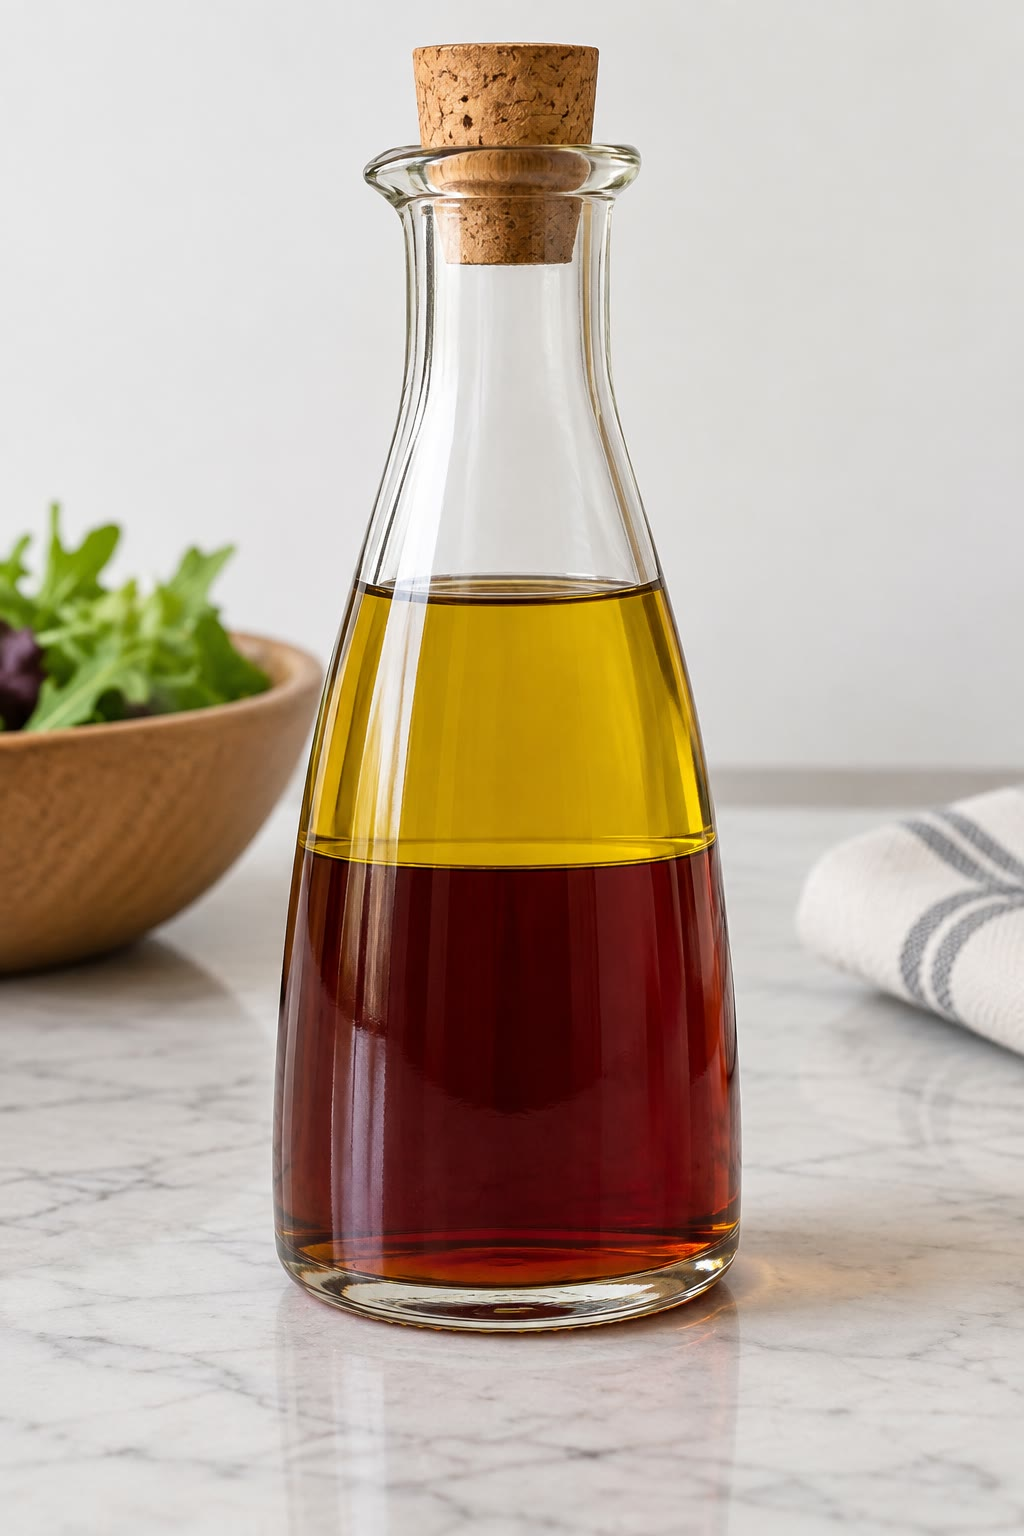
\includegraphics[width=0.2\linewidth]{images/book2/ai/b1-04-dressing.jpg}

{\small Een slasaus in rust: olijfolie, apolair, drijft op azijn, een
waterige oplossing; de twee vloeistoffen zijn niet mengbaar.}
\end{omfigure}

\begin{definition}[Hydrofiel, hydrofoob, amfifiel]\label{def:b1:intermolecular-forces-solvents:amphiphile}
Een groep is \emph{hydrofiel}\index{hydrofiel} wanneer hij gunstig
wisselwerkt met water (ionaire of polaire groepen: \ce{-COO^-}, \ce{-OH},
\ce{-SO3^-}) en \emph{hydrofoob}\index{hydrofoob} wanneer dat niet zo is
(koolwaterstofketens). Een molecuul is \emph{amfifiel}\index{amfifiel}
wanneer het zowel een hydrofiele kop als een hydrofobe staart draagt.
\end{definition}

\begin{example}[Zeep]\label{ex:b1:intermolecular-forces-solvents:soap}
Natriumdodecanoaat, \ce{CH3(CH2)10COO- Na+}, is \omterm{def:b1:intermolecular-forces-solvents:amphiphile}{amfifiel}. Aan het
wateroppervlak staan de moleculen met de kop in het water en de staart in
de lucht. In het inwendige van het water, boven een kleine concentratie,
groeperen ze zich tot bolletjes --- micellen --- met de staarten binnenin
en de koppen buiten. Vet, dat apolair is, lost op in de \omterm{def:b1:intermolecular-forces-solvents:amphiphile}{hydrofobe} kern
van de micellen en wordt door het water afgevoerd.
\end{example}

\begin{omfigure}
\begin{tikzpicture}[font=\small]
  % interface
  \fill[omWater] (-3.2,-1.6) rectangle (-0.4,0);
  \draw[omDef!60] (-3.2,0) -- (-0.4,0);
  \node[anchor=south west] at (-3.2,0.95) {lucht};
  \node[anchor=north west] at (-3.2,-1.2) {water};
  \foreach \x in {-2.9,-2.5,...,-0.6} {
    \fill[omThm] (\x,-0.12) circle (0.11);
    \draw[thick, black!70, decorate, decoration={zigzag, amplitude=1pt, segment length=3pt}] (\x,0) -- (\x,0.85);
  }
  % micelle
  \begin{scope}[xshift=3.2cm, yshift=-0.4cm]
    \fill[omWater] (-2,-1.6) rectangle (2,1.6);
    \foreach \a in {0,30,...,330} {
      \draw[thick, black!70, decorate, decoration={zigzag, amplitude=1pt, segment length=3pt}] (\a:0.25) -- (\a:1.0);
      \fill[omThm] (\a:1.12) circle (0.11);
    }
    \node[anchor=north] at (0,-1.65) {een micel in water};
  \end{scope}
\end{tikzpicture}

{\small \omterm{def:b1:intermolecular-forces-solvents:amphiphile}{Amfifiele} moleculen (rode \omterm{def:b1:intermolecular-forces-solvents:amphiphile}{hydrofiele} kop, zigzaggende \omterm{def:b1:intermolecular-forces-solvents:amphiphile}{hydrofobe}
staart) aan het wateroppervlak en gegroepeerd tot een micel, in
doorsnede getekend; micellen worden bestudeerd in het deel van jaar 3.}
\end{omfigure}

\begin{method}[Een oplosmiddel kiezen]\label{met:b1:intermolecular-forces-solvents:choose}
Zo kies je een oplosmiddel voor een opgeloste stof of een reactie:
\begin{enumerate}
  \item karakteriseer de opgeloste stof: ionair, polair, in staat om
        \omterm{def:b1:intermolecular-forces-solvents:hbond}{waterstofbruggen} te geven of op te nemen, of apolair;
  \item kies een oplosmiddel van dezelfde soort (\cref{prop:b1:intermolecular-forces-solvents:like}),
        met een hoge permittiviteit als er ionen gescheiden moeten worden;
  \item kies voor een reactie tussen een anion en een molecuul bij
        voorkeur een polair \omterm{def:b1:intermolecular-forces-solvents:solvent-classes}{aprotisch oplosmiddel}, dat het zout oplost
        zonder het anion met \omterm{def:b1:intermolecular-forces-solvents:hbond}{waterstofbruggen} te binden
        (\cref{ch:b1:nucleophilic-substitution});
  \item kies voor een extractie een oplosmiddel dat niet mengbaar is met
        het eerste en waarin de opgeloste stof veel beter oplost.
\end{enumerate}
\end{method}

\section{Oefeningen}

\begin{exercise}[$\star$]\label{exo:b1:intermolecular-forces-solvents:1}
Noem de interacties tussen de deeltjes van vloeibaar argon, vloeibaar
waterstofchloride, vloeibaar water, vloeibaar methaan en vast dijood, en
zeg welke in elk geval overheerst.
\end{exercise}

\begin{exercise}[$\star$]\label{exo:b1:intermolecular-forces-solvents:2}
Welke van deze stoffen vormen \omterm{def:b1:intermolecular-forces-solvents:hbond}{waterstofbruggen} tussen hun eigen
moleculen: \ce{CH3OH}, \ce{CH3OCH3}, \ce{CH3NH2}, \ce{CH3F}, \ce{HF},
\ce{CH4}? Welke kunnen alleen \omterm{def:b1:intermolecular-forces-solvents:hbond}{waterstofbruggen} van een ander molecuul
opnemen?
\end{exercise}

\begin{exercise}[$\star$]\label{exo:b1:intermolecular-forces-solvents:3}
Deel met de tabel van oplosmiddelen water, ethanol, propanon, hexaan,
dichloormethaan en acetonitril in als polair of apolair, protisch of
aprotisch.
\end{exercise}

\begin{exercise}[$\star$]\label{exo:b1:intermolecular-forces-solvents:4}
Leg uit waarom dijood veel beter oplost in hexaan dan in water, en
waarom natriumchloride zich omgekeerd gedraagt.
\end{exercise}

\begin{exercise}[$\star\star$]\label{exo:b1:intermolecular-forces-solvents:5}
Methanol kookt bij \qty{64.7}{\celsius}, ethanol bij \qty{78.4}{\celsius},
ethaanzuur bij \qty{118.1}{\celsius} en methoxymethaan bij
\qty{-25.0}{\celsius}. Verklaar de volgorde.
% ledger: bp:CH3OH, bp:C2H5OH, bp:CH3COOH, bp:CH3OCH3
\end{exercise}


\begin{exercise}[$\star\star$]\label{exo:b1:intermolecular-forces-solvents:6}
Bereken de coulombkracht tussen een \ce{Na+}- en een \ce{Cl-}-ion op
\qty{500}{pm} van elkaar in vacuüm ($\varepsilon_0 = \qty{8.854e-12}{F/m}$,
$e = \qty{1.602e-19}{C}$), daarna in water ($\varepsilon_r = 78.4$) en in
hexaan ($\varepsilon_r = 1.89$). Becommentarieer.
\end{exercise}

\begin{exercise}[$\star\star$]\label{exo:b1:intermolecular-forces-solvents:7}
Propanon en water zijn in alle verhoudingen \omterm{def:b1:intermolecular-forces-solvents:miscibility}{mengbaar}; hexaan en water
niet. Verklaar dit aan de hand van de interacties die verbroken en
gevormd worden.
\end{exercise}

\begin{exercise}[$\star\star$]\label{exo:b1:intermolecular-forces-solvents:8}
\ce{HCl} heeft een \omterm{def:b1:lewis-resonance-vsepr:dipole}{dipoolmoment} van \qty{1.09}{\debye} en kookt bij
\qty{-85.0}{\celsius}; \ce{HBr} heeft \qty{0.83}{\debye} en kookt bij
\qty{-66.4}{\celsius}. Waarom kookt het minder \omterm{def:b1:lewis-resonance-vsepr:dipole}{polaire molecuul} hoger?
% ledger: dip:HCl, dip:HBr, bp:HCl, bp:HBr
\end{exercise}


\begin{exercise}[$\star\star$]\label{exo:b1:intermolecular-forces-solvents:9}
Teken het cyclische dimeer van ethaanzuur. In oplossing in benzeen
gedraagt ethaanzuur zich alsof zijn molaire massa ongeveer twee keer
\qty{60}{g/mol} is; in water niet. Verklaar beide feiten.
\end{exercise}

\begin{exercise}[$\star\star\star$]\label{exo:b1:intermolecular-forces-solvents:10}
Beschrijf het oplossen van natriumchloride in water aan de hand van
dissociatie en \omterm{def:b1:intermolecular-forces-solvents:dissolution}{solvatatie}, en dat van waterstofchloride in water in
termen van ionisatie, dissociatie en \omterm{def:b1:intermolecular-forces-solvents:dissolution}{solvatatie}. Waarom geeft
waterstofchloride in hexaan een niet-geleidende oplossing?
\end{exercise}

\begin{exercise}[$\star\star\star$]\label{exo:b1:intermolecular-forces-solvents:11}
Bereken uit de kookpunten van de onvertakte alkanen (pentaan
\qty{36.1}{\celsius}, decaan \qty{174.1}{\celsius}) de gemiddelde
toename per \ce{CH2}-groep tussen \ce{C5} en \ce{C10}, en schat het
kookpunt van undecaan. Waarom wordt de toename kleiner langs de reeks?
% ledger: bp:C5H12, bp:C10H22
\end{exercise}


\begin{exercise}[$\star\star\star$]\label{exo:b1:intermolecular-forces-solvents:12}
Natriumdodecylsulfaat, \ce{CH3(CH2)11OSO3^- Na+}, is een detergent. Wijs
het \omterm{def:b1:intermolecular-forces-solvents:amphiphile}{hydrofiele} en het \omterm{def:b1:intermolecular-forces-solvents:amphiphile}{hydrofobe} deel aan, schets de schikking van de
moleculen aan het wateroppervlak en in een micel, en leg uit hoe het een
olievlek uit een stof verwijdert.
\end{exercise}

\section{Probleem: als water geen waterstofbruggen had}

\begin{problem}[{Weekendprobleem --- londonkrachten in de edelgassen en
de alkanen, de keuze van een oplosmiddel, en het kookpunt dat water
zonder waterstofbruggen zou hebben}]
\label{pb:b1:intermolecular-forces-solvents:1}
Kookpunten onder \qty{1}{atm} (in \unit{\celsius}): \ce{He} $-268.9$,
\ce{Ne} $-246.1$, \ce{Ar} $-185.9$, \ce{Kr} $-153.4$, \ce{Xe} $-108.1$;
pentaan 36.1, hexaan 68.8; \ce{CH4} $-161.5$, \ce{SiH4} $-112.0$,
\ce{GeH4} $-88.1$; \ce{NH3} $-33.4$, \ce{PH3} $-87.8$, \ce{AsH3} $-62.5$;
\ce{H2O} 100.0, \ce{H2S} $-60.3$, \ce{H2Se} $-41.3$; \ce{HF} 19.6,
\ce{HCl} $-85.0$, \ce{HBr} $-66.4$.
% ledger: bp:He, bp:Ne, bp:Ar, bp:Kr, bp:Xe, bp:C5H12, bp:C6H14, bp:CH4,
% bp:SiH4, bp:GeH4, bp:NH3, bp:PH3, bp:AsH3, bp:H2O, bp:H2S, bp:H2Se,
% bp:HF, bp:HCl, bp:HBr

\medskip
\noindent\textbf{Deel I --- Alleen London.}
\begin{enumerate}
  \item Welke interactie houdt de atomen van vloeibaar argon bijeen?
  \item Verklaar de stijging van het kookpunt van helium tot xenon.
  \item Waarom is het kookpunt van helium het laagste van alle stoffen?
  \item Vergelijk pentaan en hexaan: wat voegt één \ce{CH2}-groep toe?
  \item Methaan, silaan en germaan hebben geen \omterm{def:b1:lewis-resonance-vsepr:dipole}{dipoolmoment}. Welke
        interactie verklaart de volgorde van hun kookpunten?
  \item Waarom is in methaan geen \omterm{def:b1:intermolecular-forces-solvents:hbond}{waterstofbrug} mogelijk?
\end{enumerate}

\medskip
\noindent\textbf{Deel II --- Oplosmiddelen kiezen.}
Gebruik de tabel van oplosmiddelen van het hoofdstuk.
\begin{enumerate}[resume]
  \item Welk oplosmiddel uit de tabel lost natriumchloride het best op, en
        waarom?
  \item Met welke factor is de aantrekking tussen twee ionen op dezelfde
        afstand kleiner in water dan in hexaan?
  \item Een reactie tussen het anion \ce{CN-} en een organisch molecuul
        moet worden uitgevoerd in een oplosmiddel dat het zout oplost maar
        het anion niet met \omterm{def:b1:intermolecular-forces-solvents:hbond}{waterstofbruggen} bindt. Kies er een.
  \item Welk oplosmiddel uit de tabel zou je kiezen om dijood uit een
        waterige oplossing te extraheren, en in welke laag komt het jood
        terecht?
  \item Leg uit waarom ethanol niet voor die extractie gebruikt kan
        worden.
  \item Ethoxyethaan is nauwelijks \omterm{def:b1:intermolecular-forces-solvents:miscibility}{mengbaar} met water, hoewel het polair
        is. Stel een verklaring voor.
\end{enumerate}

\medskip
\noindent\textbf{Deel III --- De andere hydriden.}
\begin{enumerate}[resume]
  \item Bereken voor \omterm{def:b1:periodicity:table}{groep} 17 de verandering van het kookpunt van \ce{HCl}
        naar \ce{HBr}, en extrapoleer dezelfde verandering terug naar
        \omterm{def:b1:periodicity:table}{periode} 2.
  \item Vergelijk de geëxtrapoleerde waarde met het kookpunt van \ce{HF}.
  \item Dezelfde twee vragen voor \omterm{def:b1:periodicity:table}{groep} 15 (\ce{PH3}, \ce{AsH3} en
        \ce{NH3}).
  \item Ligt \ce{CH4} voor \omterm{def:b1:periodicity:table}{groep} 14 boven of onder de extrapolatie vanuit
        \ce{SiH4} en \ce{GeH4}? Waarom is dat niet verrassend?
  \item Rangschik de overschotten van \ce{NH3}, \ce{HF} en water.
  \item Tel de \omterm{def:b1:intermolecular-forces-solvents:hbond}{waterstofbruggen} die elk molecuul \ce{NH3}, \ce{HF} en
        \ce{H2O} kan geven en opnemen, en verklaar de rangorde.
\end{enumerate}

\medskip
\noindent\textbf{Deel IV --- Water zonder \omterm{def:b1:intermolecular-forces-solvents:hbond}{waterstofbruggen}.}
\begin{enumerate}[resume]
  \item Waarom zijn \ce{H2S} en \ce{H2Se} geschikt voor een extrapolatie,
        en water zelf niet?
  \item Bereken de verandering van het kookpunt van \ce{H2S} naar
        \ce{H2Se}.
  \item Stel de vergelijking op van de rechte door deze twee punten, met
        de \omterm{def:b1:periodicity:table}{periode} $p$ als variabele.
  \item Leid het kookpunt af dat water bij $p = 2$ zou hebben.
  \item Met hoeveel verhogen \omterm{def:b1:intermolecular-forces-solvents:hbond}{waterstofbruggen} het kookpunt van water?
  \item Besluit: bij welke temperatuur zou water koken als zijn moleculen
        elkaar aantrokken zoals die van \ce{H2S}?
\end{enumerate}
\end{problem}
